\chapter{Discussion of Experimental Errors}
\label{Errors}
All sources of error in this study can be classified into three groups: \begin{enumerate*}[font={\color{red!50!black}\bfseries}]

\item \textbf{Resolution of measurement}, a source of random error reflective of the precision of particle ToF and position measurements,
\item \textbf{Counting error}, another a source of random error, and lastly,
\item \textbf{Systematic errors}, the mitigation of which has motivated detector design and new methods for data analysis.

\end{enumerate*}
\vspace{-4mm}
\section{Random Errors}
\subsection{Resolution of measurement}
The position of a detected particle is known to within a specified resolution, which translates into a resolution in the measurement of the opening angle between a pair of particles.
A particle's reconstructed position along a detector lengthwise is achieved by using the timing difference between two PMTs, producing a result known to within $\pm$13 cm.\todo{Use my plot on wiki of PMT diff with Co60 at the center. Use this to deduce the vertical position uncertainty.}
Due to the detector's 15 cm width, there is also a positional uncertainty of $\pm 7.5$ cm in the direction perpendicular to the detector's length.
The amount of uncertainty in a two-neutron opening angle measurement is a function of the uncertainty in the positions of each neutron.
This function is determined by the propagation of the positional uncertainties through the formula for the calculation of opening angle, which is given by
\begin{displaymath}
    \theta_{nn} = \text{arccos}\left(\frac{\vec{v_{1}}^{\,}\cdot\vec{v_{2}}^{\,}}{|\vec{v_{1}}^{\,}||\vec{v_{2}}^{\,}|}\right)
\end{displaymath}
where $\vec{v_{1}}^{\,} = (x_1,y_1,z_1)$ and $\vec{v_{2}}^{\,} = (x_2,y_2,z_2)$ are the detected positions of the two neutrons.
The propagation of error through this formula is achieved by evaluating the following expression
\begin{eqnarray*}
 \Delta \theta_{nn} & = & \left( \left(\Delta x_1 \frac{\partial \theta}{\partial x_1}\right)^{2} + \left(\Delta y_1 \frac{\partial \theta}{\partial y_1}\right)^{2} + \left(\Delta z_1 \frac{\partial \theta}{\partial z_1}\right)^{2} + \right. \\
 & & \left. + \left(\Delta x_2 \frac{\partial \theta}{\partial x_2}\right)^{2} + \left(\Delta y_2\frac{\partial \theta}{\partial y_2}\right)^{2} + \left(\Delta z_2 \frac{\partial \theta}{\partial z_2}\right)^{2} \right) ^{\frac{1}{2}}
\end{eqnarray*}
\todo{Mention what the deltas are in this big formula.}
Then, by using a set of opening angle bins, the average is computed of the propagated uncertainties of the measurements in each bin.
The result, seen in fig~\ref{fig:OpeningAngleRes}, can be interpreted as the opening angle resolution as a function of $\theta$.
\begin{figure}[h]
    \centering
    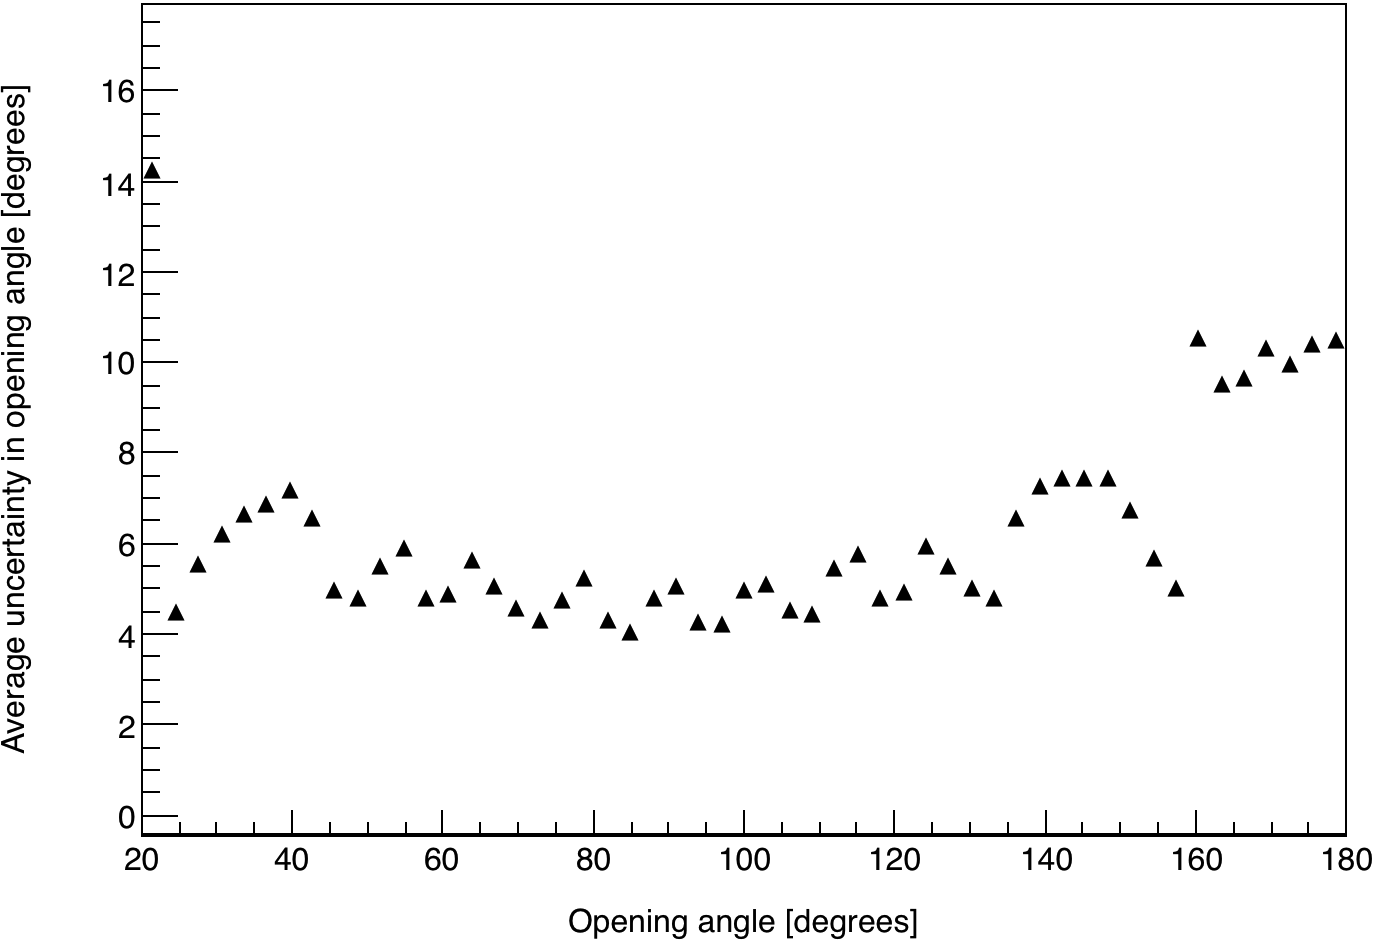
\includegraphics[width = 0.75\textwidth]{Content/Errors/OpeningAngleUncertainty.png}
    \caption{Uncertainties in opening angle as determined by the propagation of position uncertainties through the opening angle calculation.
    Because the uncertainty of a given opening angle measurement varies depending on which two detectors are involved, an average of the calculated uncertainties of measurements falling within each bin is taken.
    The y-axis can be viewed as a measure of the angular resolution in the sense that it represents the smallest angular difference that can be considered statistically significant.
    }
    \label{fig:OpeningAngleRes}
\end{figure}

\subsection{Counting error}
The standard deviation in the number of observed events is always assumed to be equal to $\sqrt{N}$, as per poissonian  statistics, were N is the number of observed events.
Opening angle measurements are separated into three different neutron energy ranges and then placed into bins 10 degrees wide.
These groups each contain between 100 and 200 events, producing a relative error between 10 and 7 percent, respectively.
The vertical error bars seen in the results are solely a reflection of such counting error.

\section{Systematic errors}
This study reports two-neutron opening angle distributions expressed as a ratio between a correlated distribution and an uncorrelated distribution in which the same set of neutron events are used to form both distributions.
In doing so, the result is unaffected by the absolute neutron efficiencies and thresholds of each detector, drifting of the high voltage supplied to the PMTs, and the geometrical acceptance of the detector array as a function of opening angle.
Furthermore, \textit{accidental} two-neutron events, which lead to an over estimation of the isotropic component of the opening angular distribution, are subtracted from the data.
\textit{Accidental} two-neutron events are defined as the detection of two causally uncorrelated events in the same pulse if both events occur during the neutron ToF window.
The subtraction of such events is possible under the assumption that the number of detected accidentals per pulse follows the poissonian distribution.
See section~\ref{Analysis} for a detailed discussion on how the subtraction is accomplished.
The validity of this assumption can be tested with measurements taken while using D$_2$O as a target.
All coincident neutrons observed from the photo-disintegration of deuterium are accidentals because only one neutron is produced per disintegration.
Figure~\ref{fig:PoissonianFits}a shows that a poissonian model gives a good fit to the distribution of the number of neurons detected in coincidence while using a D2O target.
When observing neutrons from photofission, on the other hand, there is the inclusion of correlated neutrons, together with accidental neutrons caused by multiple fissions or $(\gamma, n)$ reactions, so a poissonian model underestimates the rate of two-neutron coincidence.
See fig~\ref{fig:PoissonianFits}.
\begin{figure}[htbp]
    \centering
    \subfloat[D$_2$O target: prob near 1.0, good compatibility.]{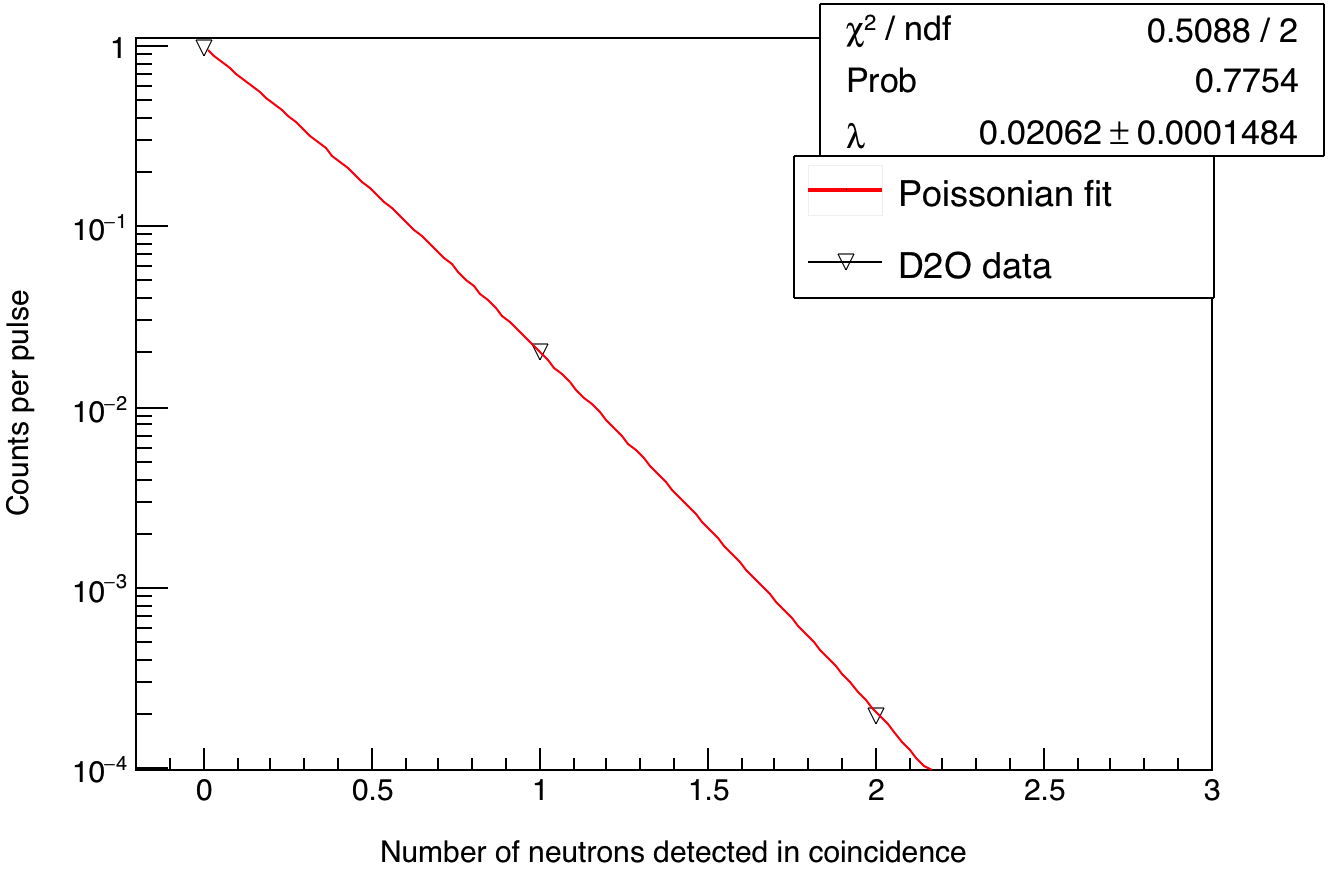
\includegraphics[width=0.55\textwidth]{Content/Errors/PoissonianFitD2O.png}}
    \subfloat[DU target: prob near 0, poor compatibility.]{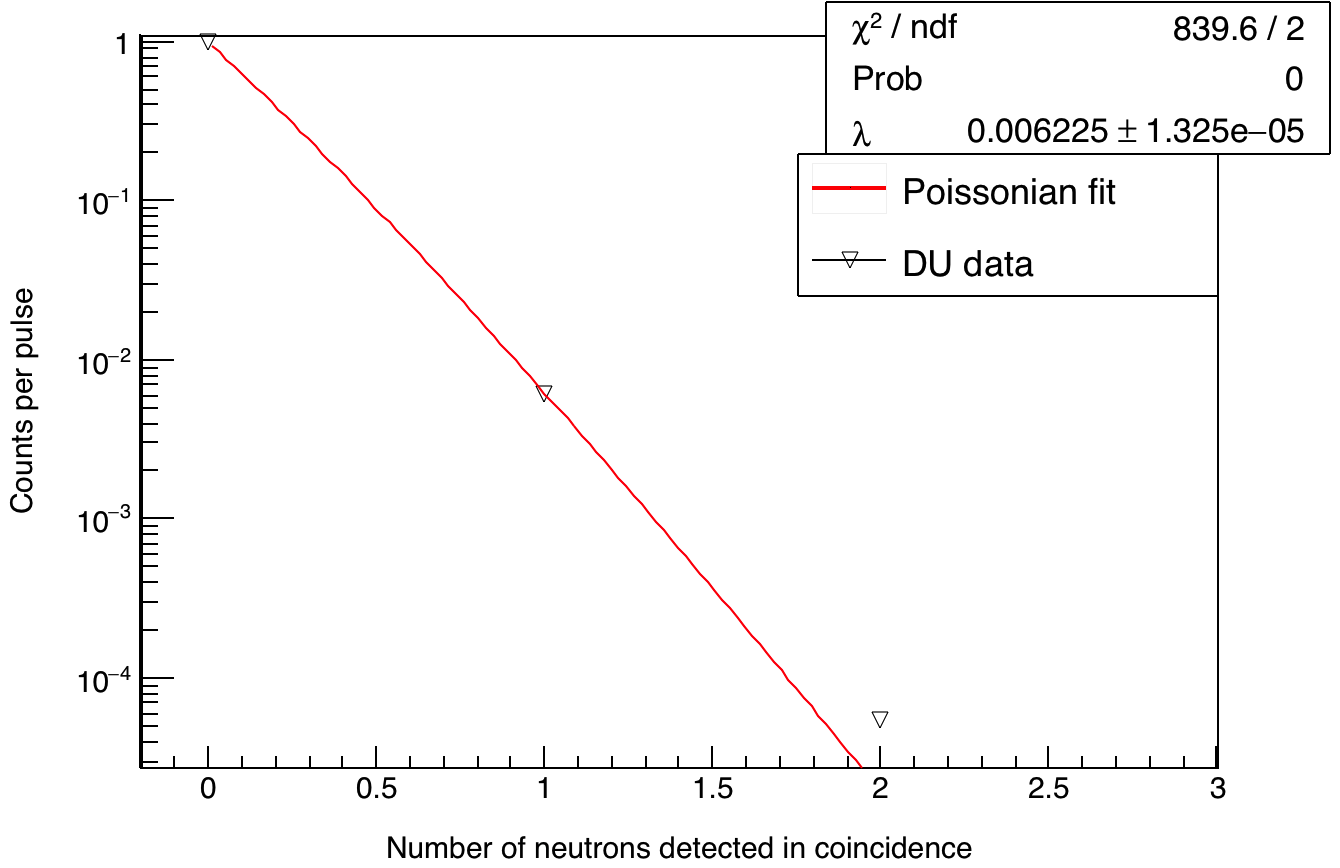
\includegraphics[width = 0.55\textwidth]{Content/Errors/PoissonianFitDU.png}}
    \caption{A D$_2$O target (left) produces only accidental neutrons, so a poissonian model is suitable.
    The p-value, denoted ``prob" on the plot, is a metric for assessing the compatibility of the data to a given model, poissonian in this case.
    A p-value of 0.77 for the D$_2$O target indicates relatively good compatibility.
    On the other hand, when using DU as a target (right), the introduction of correlated neutrons causes the poissonian model to under estimate the double-coincidence rate.
    The assumption that the coincidence rates of accidental neutrons follow the poissonian distribution is used to subtract accidentals from the data, removing this source of systematic error.}
    \label{fig:PoissonianFits}
\end{figure}

\subsection{Detector Cross-talk}
\label{crosstalk}
\textit{Cross-talk} is an undesirable phenomenon that occurs when a particle is detected in one detector, and then by any means (\textit{e.g.}\ elastic scattering), the same particle is detected in a different detector.
If both detections occur within the time frame typical for neutrons, then the cross-talk event cannot be distinguished from a true neutron coincidence.
The geometry of the neutron detector array makes it kinematically impossible for a neutron to scatter from a proton in one detector--which is the basis for scintillation--and then travel directly to another detector with enough kenetic energy to be detected.
Rather, in order for cross-talk to occur, it is required that the neutron scatter from at least one intermediate nucleus while traveling between detectors.
This fact, which can be derived from the conservation of energy and momentum, makes cross-talk a "second-order" effect, because upon depositing enough energy to be detected in one detector, the neutron must then 1) scatter from an intermediate nucleus, and 2) be detected in a second detector.
\begin{figure}
    \centering
    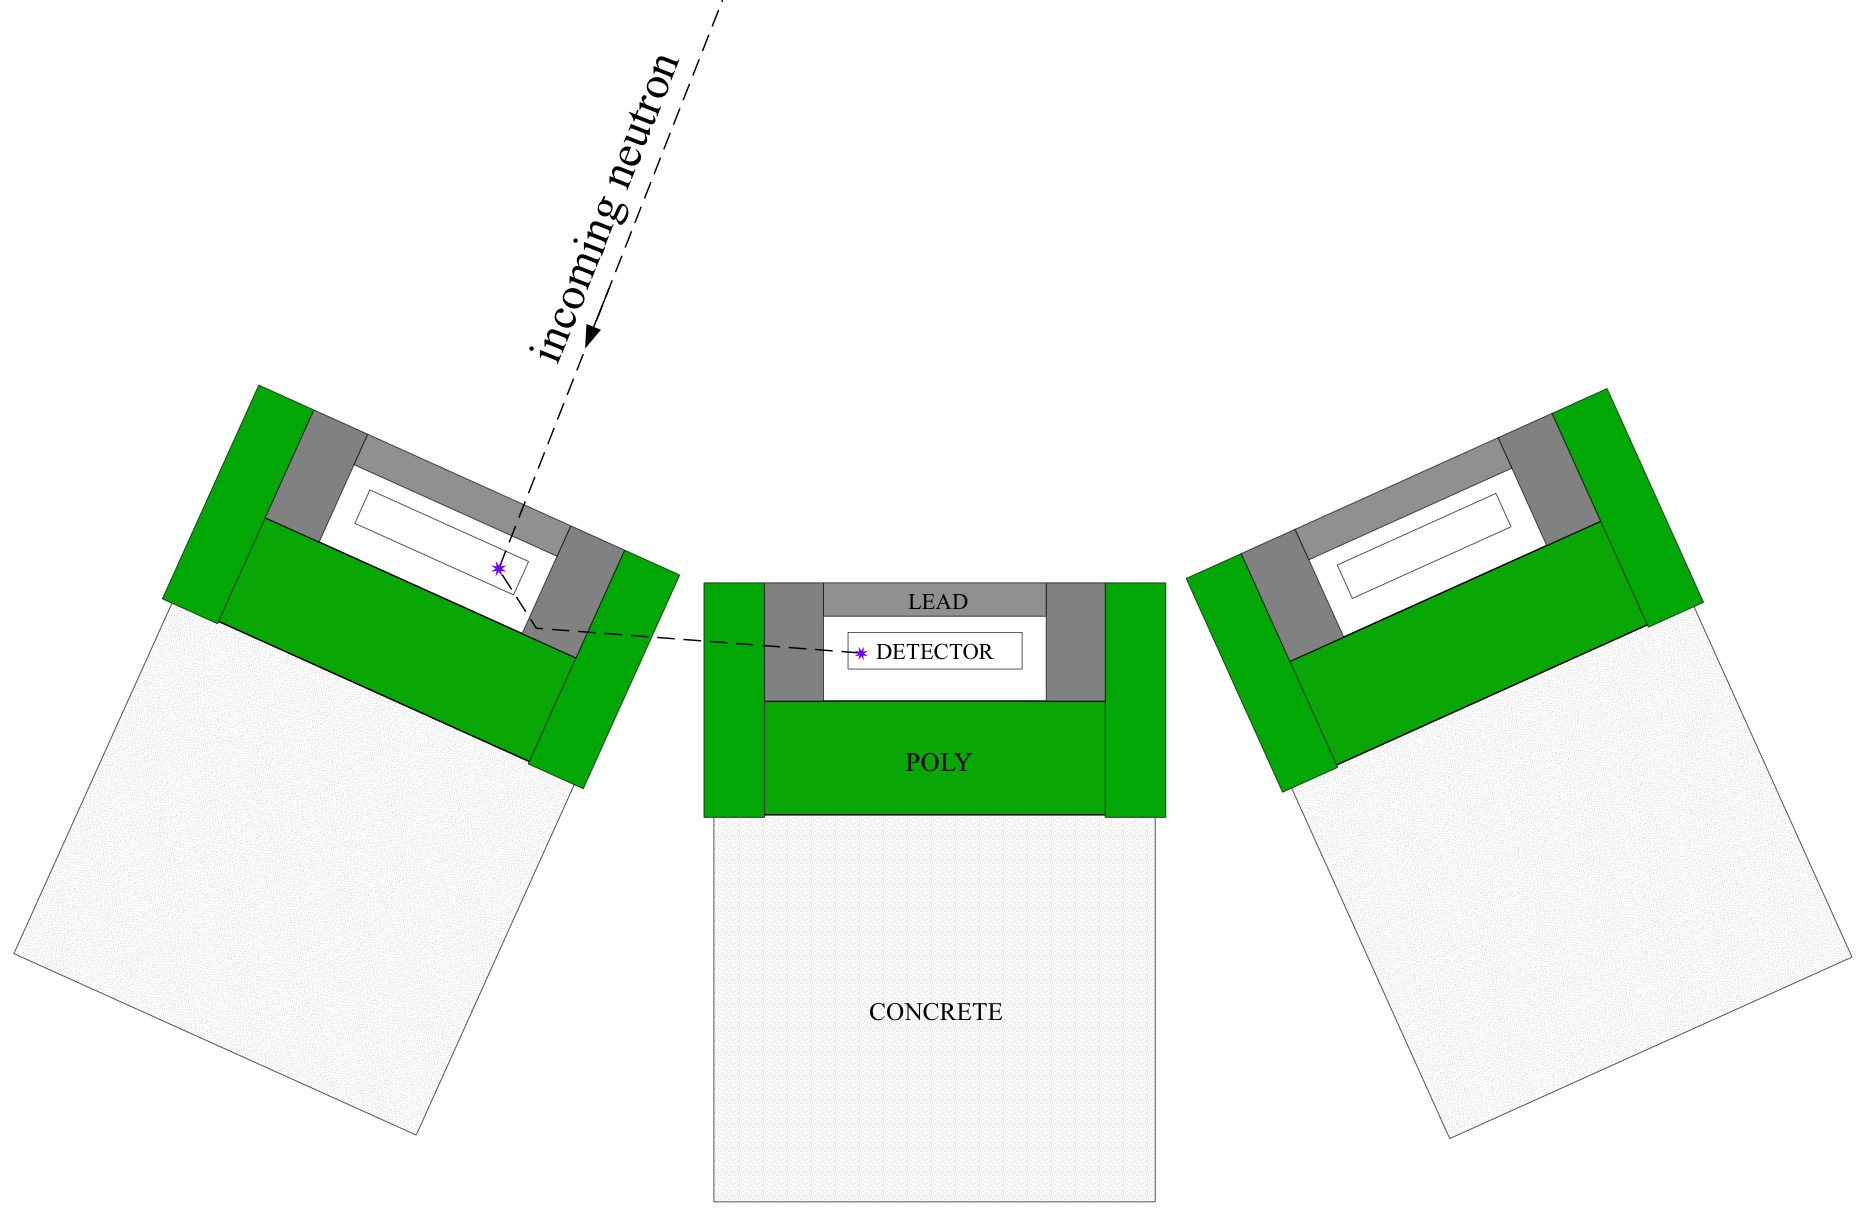
\includegraphics[width = 0.75\textwidth]{Content/Errors/CrossTalkExample.png}
    \caption{A hypothetical example of a neutron cross-talk event.
First, an incoming neutron enters a detector and is detected as the result of a collision with a proton.
Next, it scatters from some lead shielding nearby, which changes its direction of travel such that it enters a second detector where it is detected a second time.
The scattering of a neutron from an intermediate nucleus, in this case a lead nucleus in the detector's shielding, is kinematically required in order for cross-talk to occur in this experiment.}
    \label{fig:CrossTalkExamplepng}
\end{figure}
\todo[noline]{ToDo: include the other plot once the god dam wiki is back up.}
However, the fact that cross-talk is a second-order effect is not sufficient to make the claim that cross-talk is negligible,
because the detectors and their shielding contain significant levels of carbon, lead, and other nuclei which can function as intermediate scattering points.
To address this, a detailed MCNP-PoliMi~\cite{MCNP_POLIMI} simulation was performed that includes the entire array of neutron detectors, along with their shielding, supporting structures, and the concrete composing the experimental cell which contains the detectors.
PoliMi is an extension to MCNP that was developed to simulate correlated fission particles and their subsequent interactions as accurately as possible.
PoliMi includes multiplicity distributions for neutrons, photons, and the correct correlated photon production from neutron interactions.
These features are in contrast to the standard release of MCNP which uses uncorrelated distributions and average multiplicities.
As a result, the standard release of MCNP converges to the correct average result quicker than if correlated event-by-event distributions were used.
Another feature PoliMi provides is the ability for particle tracking data to be printed and post processed by the user.
Here, the particle tracking data is used to model detector physics in order to estimate the ratio of the rate of cross-talk to the rate of the detection of correlated neutrons.
Neutron detection physics was modeled by converting the amount of energy deposited by neutrons into scintillation light output, and did not include the propagation or detection of scintillation light.
The scintillation light output is given in MeV equivalent electron energy, denoted MeVee.
Neutron energy deposited from collisions with hydrogen and carbon nuclei is the only input used to calculate light output, the procedures of which are taken from ref~\cite{POLIMI}.
For neutron collisions with hydrogen, the light output in MeVee, $L$, is given by the following empirical relationship
\begin{displaymath}
L = 0.0364 E_n^2 +  0.125 E_n
\end{displaymath}
where $E_n$ is equal to the change in the kinetic energy of the neutron during the collision.
Neutron interactions with carbon are assumed to generate a smaller light output of
\begin{displaymath}
L = 0.02 E_n
\end{displaymath}
The simulation used MCNP-PoliMi's built in $^{252}$Cf spontaneous fission source, which emits neutrons with the correct correlations.
The light output threshold for detection was set empirically by choosing the threshold that gave the best agreement between the ToF spectra of simulation and measurement (see fig~\ref{fig:Cf252MCNPVsEXP}).
\begin{figure}
    \centering
    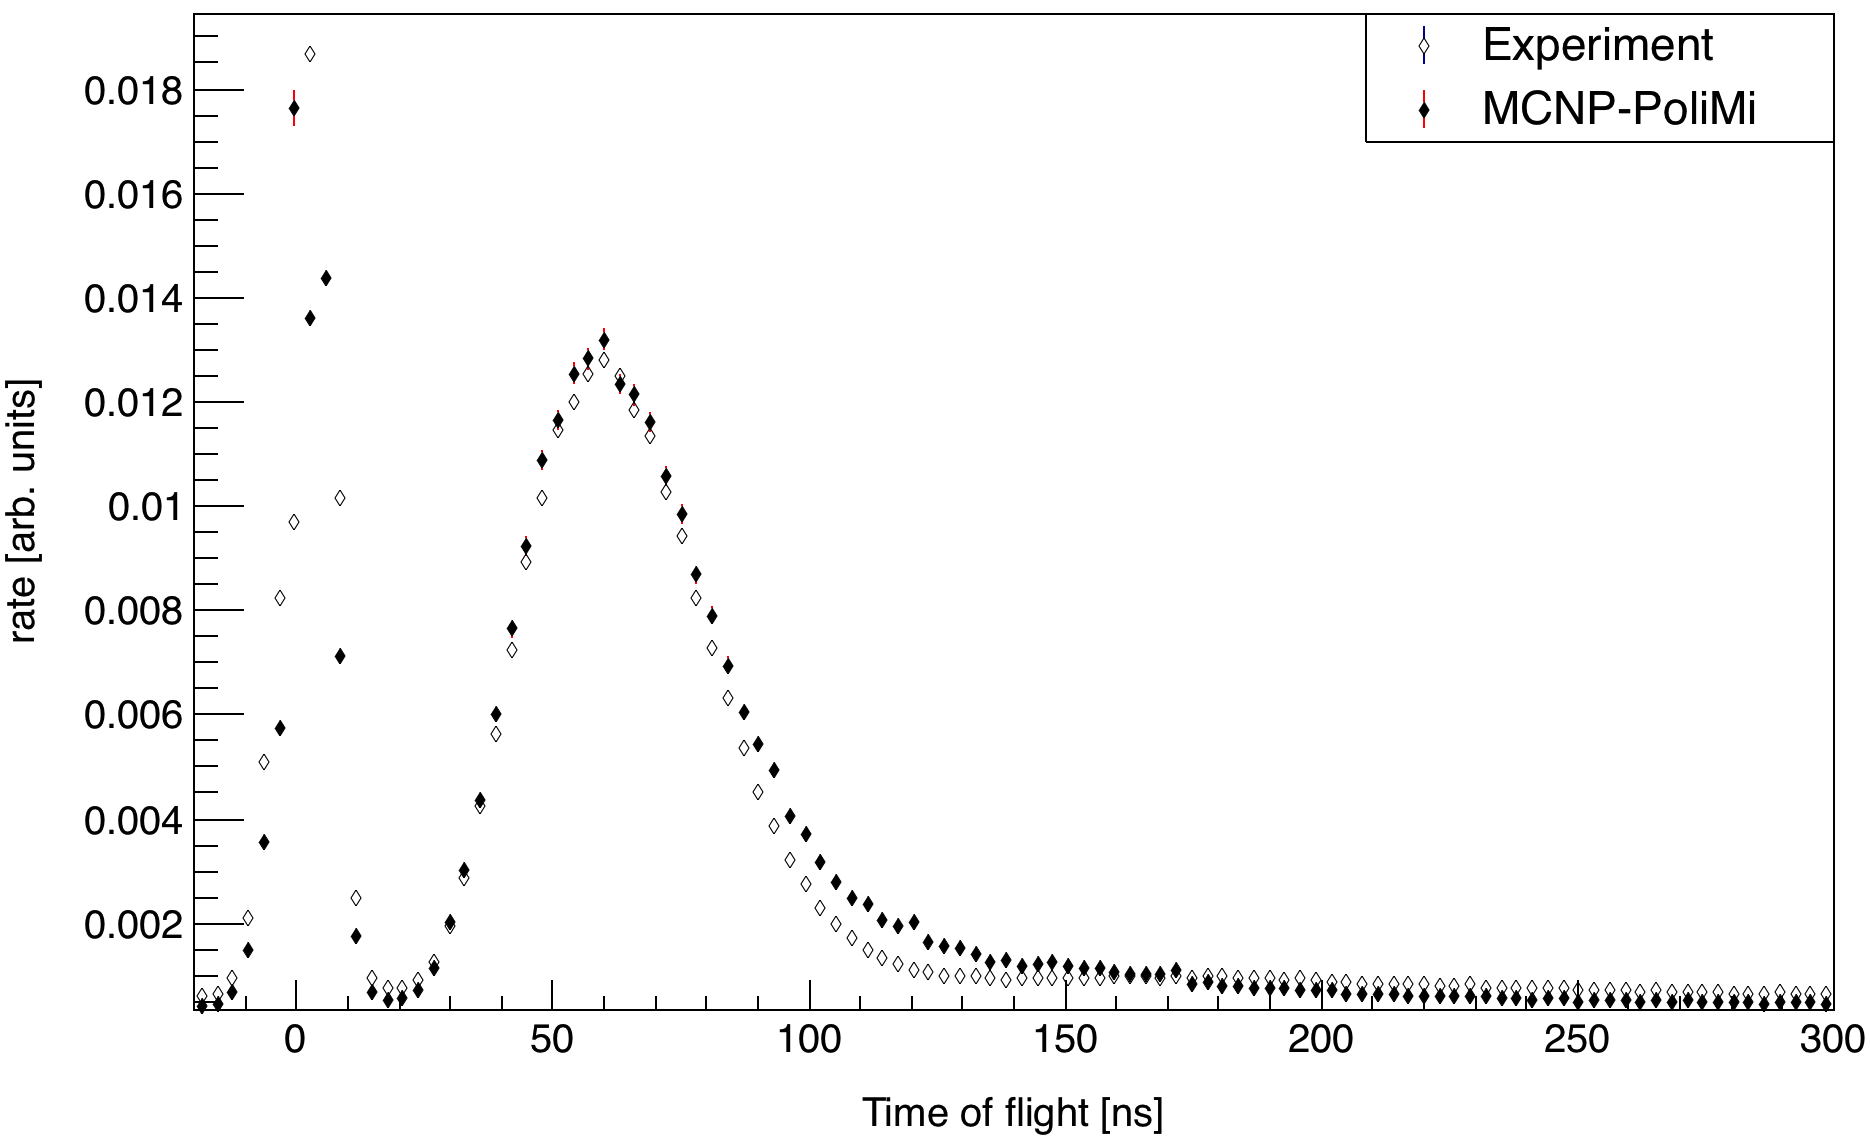
\includegraphics[width = 0.9\textwidth]{Content/Errors/Cf252MCNPVsEXP.png}
    \caption{Measured vs simulated ToF spectrum of a $^{252}$Cf spontaneous fission source.
    In the simulation, the light output threshold for detection was varied until the result was in good agreement with measurement.}
    \label{fig:Cf252MCNPVsEXP}
\end{figure}
A tally is kept of the number of cross-talk events and the number of correlated neutron pairs detected.
An event is considered a "neutron event" if there is a light output of greater than 0.03 MeVee produced in a detector in a time frame of 10 ns or less.
Furthermore, the 0.03 MeVee light output threshold must be reached sometime during the neutron time of flight window used in the experiment, which is 45 to 150 ns.
This way, the method used for particle identification in the simulation mimics that which is used in the experiment.
The opening angle is calculated from the positions at which each particle produced a light output above the 0.03 MeVee threshold.
In the simulation, cross-talk events accounted for 3\% of total coincident events.
Accordingly, no cross-talk corrections were applied to the data.
Figure~\ref{fig:CrosstalkVScoincidence} shows the distribution of cross-talk events as a function of opening angle.
\begin{figure}
    \centering
    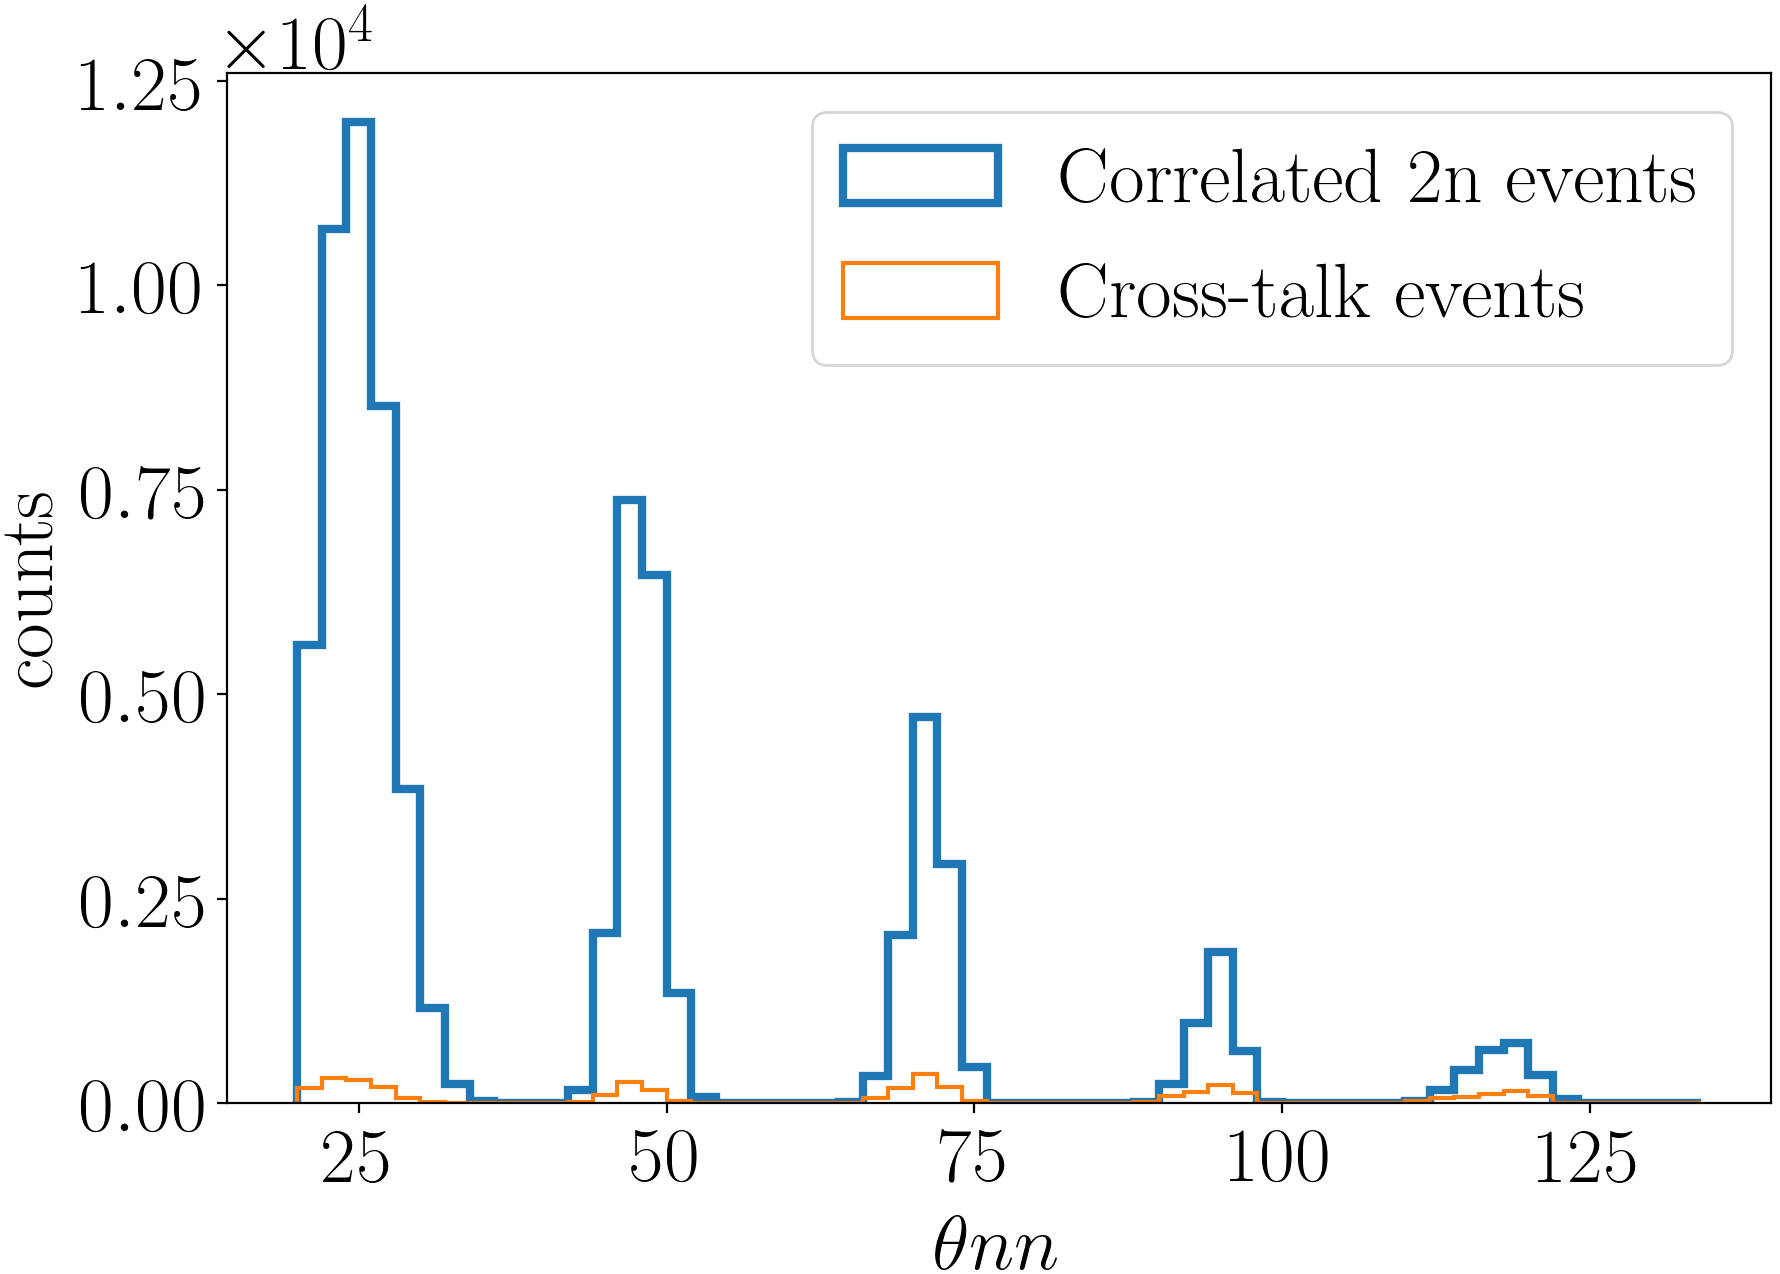
\includegraphics[width = 0.9\textwidth]{Content/Errors/CrosstalkVScoincidence.png}
    \caption{Number of cross-talk events and two-neutron coincidences as a function of opening angle.}
    \label{fig:CrosstalkVScoincidence}
\end{figure}

\subsection{Elastic Scattering in Target}
One consideration for the design of the target was the probability that fission neutrons produced in the target will scatter before exiting the target.
This is a cause for concern, because the scattering of neutrons from heavy nuclei highly alters the neutron's direction of travel, creating two-neutron opening angles that are not reflective of the true opening angle immediately after fission.
This effect cannot be completely eliminated, but the target must be small enough such that neutron scattering is negligible.
The size of such target was found by performing an MCNP simulation in which neutrons with an energy spectrum typical of fission neutrons are sampled uniformly within the target.
From the simulation, 97.5\% of the neutrons produced in a DU target with dimensions of 4x2x0.05 $\text{cm}^3$ escaped without scattering.
Two neutrons are required for the formation of an opening angle, so the rate of data contamination due to scattering is $(1-.975^2)$, or 5\% of two-neutron events.
\begin{figure}
    \centering
    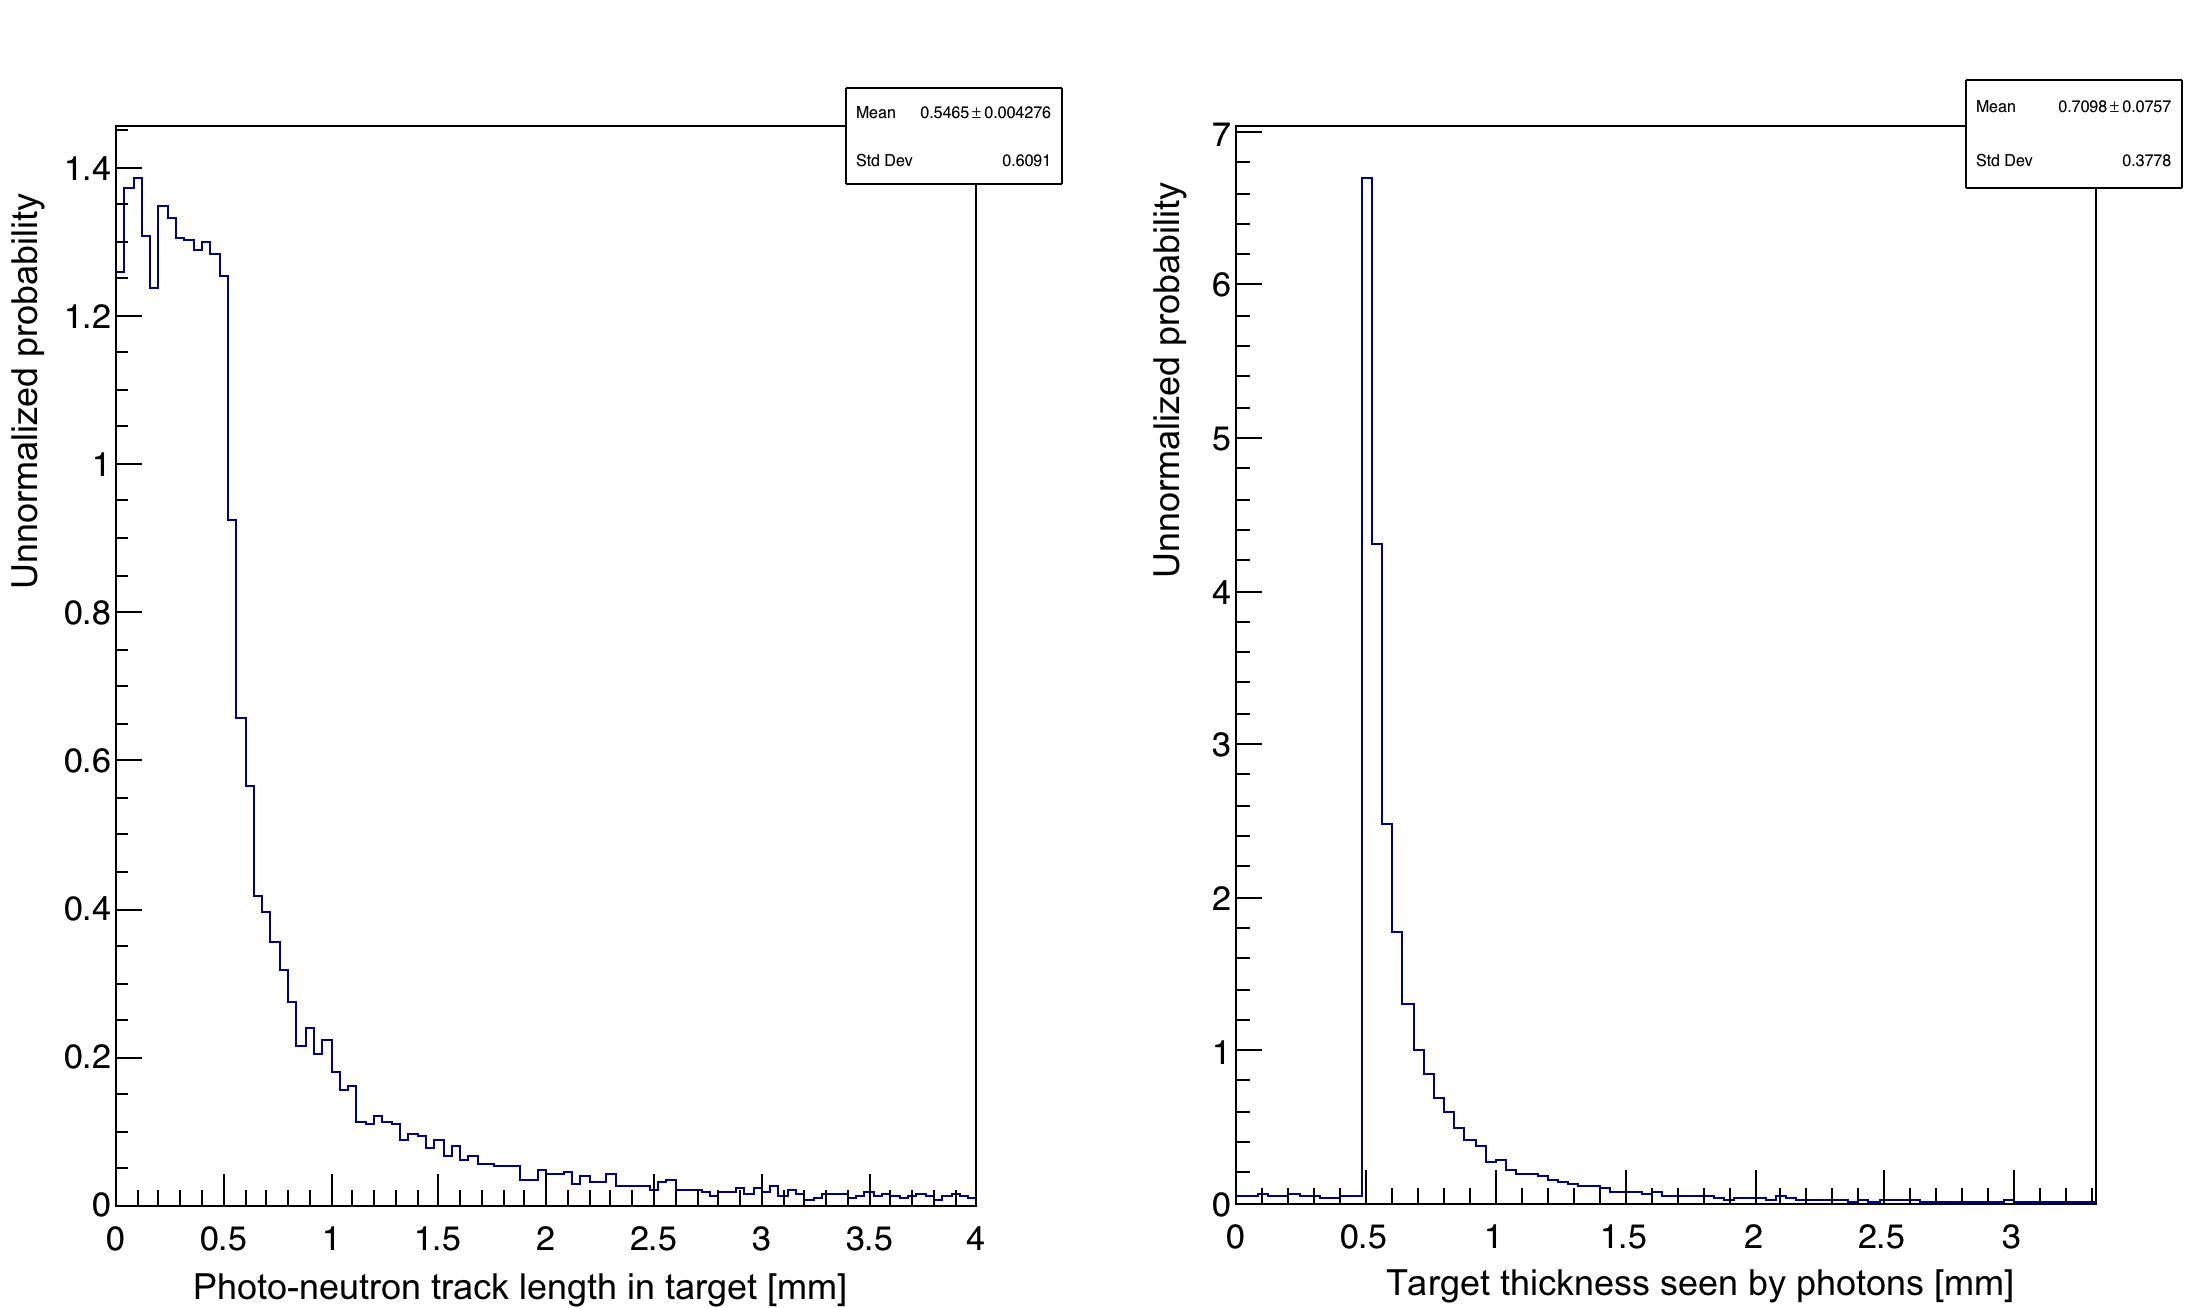
\includegraphics[width = \textwidth]{Content/Errors/ScatteringInTarget.png}
    \caption{Somehow relevant plot.}
    \label{fig:ScatteringInTarget}
\end{figure}
\todo[inline]{ToDo: Maybe expand on this section a little bit. Add the plot of contamination VS radius for Th. Do simulation for DU}
